% Letter class
\documentclass[10pt]{letter}
\usepackage[hmargin=1.5in,vmargin=1.5in]{geometry}
\usepackage{graphicx}
\usepackage{braket}

\usepackage[
    backend=biber,
    style=nature,
    % citestyle=authortitle,
    % natbib=true,
    % url=false,
    % doi=false,
    % eprint=false,
    % natbib=true,
    sorting=none,
]{biblatex}
\addbibresource{references.bib}

% Name of sender
\name{Thomas C. Fraser}

% Signature of sender
\signature{Thomas C. Fraser}

% Address of sender
\address
{
    \textbf{Thomas C. Fraser} \\
    tfraser@perimeterinstitute.ca\\
    +1 (226) 868-0557\\
    Perimeter Institute for Theoretical Physics,\\
    31 Caroline St N, Waterloo, Ontario N2L 2Y5, Canada
}


%-----------------------------------------------------------------------------%

\begin{document}

% Name and address of receiver
\begin{letter}
{
    E. Wolfe, R. Spekkens \& The Postdoc Hiring Committee,\\
    Perimeter Institute for Theoretical Physics,\\ 
    31 Caroline St N, Waterloo, Ontario N2L 2Y5, Canada.
}

\opening{For the Postdoc Hiring Committee at PI:}

I am writing to express my interest in re-joining the research group of E. Wolfe and R. Spekkens as post-doctoral student to work on the ``Quantum Causal Inference Initiative''.
In the interest of disclosing any potential conflicts of interest, I wish to inform you that I am currently a PhD Candidate working under the supervision of R. Spekkens in the Quantum Foundations group at PI and I will be graduating April of 2023.
I have also collaborated directly with E. Wolfe in the past.

\noindent\makebox[\linewidth]{\rule{6cm}{0.4pt}}

Dear E. Wolfe, R. Spekkens,

For a variety technological, ethical, environmental, or fundamental reasons, scientists are often limited in their ability to interact with and collect empirical data about the complex, multipartite systems they care about. Despite these limitations, it remains possible to make inferences about the causal relations governing the various parts of the whole system.



The quantum marginal problem (QMP) and the problem of quantum causal modelling (QCM) and closely related. 
For example, it is well-understood that a tripartite quantum state, $\rho_{ABC}$, is consistent with the causal hypothesis that system $B$ is the complete common cause of $A$ and $C$, depicted by $A \leftarrow B \rightarrow C$, if and only if its quantum conditional mutual information $I(A, C | B)$ vanishes \cite{allen2017quantum}. This condition is also equivalent to the condition that $\rho_{ABC}$ can be decomposed by splitting system $B$ such that \cite{hayden2004structure}
\begin{equation}
    \rho_{ABC} \cong {\bigoplus}_{i} p_i (\rho_{AB_i^{L}} \otimes \rho_{B_i^{R} C}).
    \nonumber
\end{equation}
At the level of the QMP, this condition stipulates that the tripartite state $\rho_{ABC}$ can be \textit{reconstructed} from the two-body marginals $\rho_{AB}$ and $\rho_{BC}$.

 the Inflation Technique has proven to be a promising tool for understanding the observational consequences of a given causal hypothesis \cite{wolfe2019inflation}.


Unsurprisingly, the QMP is connected to numerous topics in quantum information theory including quantum entanglement, quantum many-body physics, quantum error correction, quantum entropic inequalities, random matrix theory, and representation theory.

For these reasons,
\cite{fraser2022sufficient}


The primary focus of my Master's thesis~\cite{fraser2020combinatorial} was the subject of \textit{classical} causal inference. The was to switch from using tools from real algebraic geometry (e.g. non-linear quantifier elimination) to tools from combinatorics.

Another topic I'm eager to work on is causal inference starting from only marginal information~\cite{budroni2016indistinguishability}. In this restricted setting, it is also possible to prove quantum advantages for causal inference in a similar spirit to those of \cite{ried2015quantum}.

For example, starting from a pair of marginal distributions, $p_{AB}$ and $q_{BC}$ (for which $p_{B} = q_{B}$), it is impossible to distinguish between (i) the causal hypothesis that $B$ is the complete common cause of $A$ and $C$, and (ii) any saturating causal hypothesis, e.g., the hypothesis that a fourth system, $\Lambda$, is the complete common cause of $A$, $B$ and $C$.
\begin{center}
    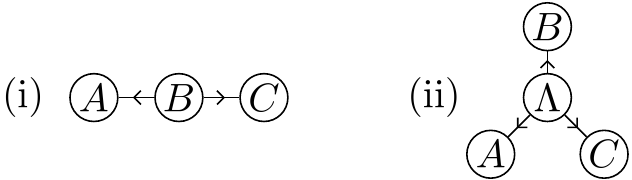
\includegraphics[scale=0.25]{common_cause_direct_cause}
\end{center}
The reason for this is simply that probability distributions are \textit{adhesive} in the sense that there always exists a joint distribution,
\begin{equation}
    r_{ABC}(abc) = \frac{p_{AB}(ab) q_{BC}(bc)}{p_{B}(b)},
\end{equation}
that is both compatible with hypothesis (i) and has marginal distributions $p_{AB}$ and $q_{BC}$. 
By contrast, from a pair of marginal quantum states, $\rho_{AB}$ and $\sigma_{BC}$ (for which $\rho_{B} = \sigma_{B}$), it is \textit{possible} to distinguish causal hypotheses (i) from (ii). For example, it is possible to show that there exists no tripartite quantum state compatible with causal hypothesis (i) that also has bipartite marginals $\rho_{AB} = \sigma_{BC} = \frac{1}{3}\ket{00}\bra{00} + \frac{2}{3} \left(\frac{\ket{01}+\ket{10}}{\sqrt{2}}\right)\left(\frac{\bra{01}+\bra{10}}{\sqrt{2}}\right)$ \cite{zhang2013conditional}.





% Closing statement
\closing{Sincerely,}

\end{letter}

\textbf{References}
\printbibliography[heading=none]{}

\end{document}
